\documentclass{article}
\usepackage[spanish,activeacute]{babel}
\usepackage[utf8]{inputenc}
\usepackage{amsmath,amsfonts,amssymb,amstext,amsthm,amscd}
\usepackage{latexsym}
\usepackage{graphicx}
\usepackage{subfig}
\usepackage{float}
\usepackage[table,xcdraw]{xcolor}
\usepackage{dcolumn}
\usepackage{bm}
\newcounter{itemR}
\usepackage{here}
\usepackage{fancyhdr}
\usepackage{multicol}
\usepackage{hyperref}
% -------------------------------------------------------------------
\usepackage{fancyhdr}
\setlength{\headheight}{15.2pt}
\usepackage[paperwidth=8.5in, paperheight=11.0in, top=1.0in, bottom=1.0in, left=1.0in, right=1.0in]{geometry}

\pagestyle{fancyplain}
\fancyhead[L,RO]{Pr\'actica $\#$8, Experimento de Millikan}
\fancyhead[C,CO]{}
\fancyhead[R,LO]{LFA3061-1}
\fancyfoot[L,RO]{\thepage}
\fancyfoot[C,CO]{Laboratorio de F\'isica, UDLAP}
\fancyfoot[R,LO]{}

% ------------------------------------------------------------------------------------------------------------------------------------------------------
% ------------------------------------------------------------------------------------------------------------------------------------------------------
% ------------------------------------------------------------------------------------------------------------------------------------------------------

\begin{document}

\fancypagestyle{plain}{
   	\renewcommand{\headrulewidth}{1pt}
   	\renewcommand{\footrulewidth}{1pt}
}

\renewcommand{\footrulewidth}{1pt}
\renewcommand{\tablename}{Tabla}

% ------------------------------------------------------------------------------------------------------------------------------------------------------
% ------------------------------------------------------------------------------------------------------------------------------------------------------
% ------------------------------------------------------------------------------------------------------------------------------------------------------

\title{Experimento de Millikan\small{Set 2}}
\author{\small{ {Nayma Itzel Garc'ia Escamilla \footnote{159845; nayma.garciaea@udlap.mx}}, {Freddy El'i Campillo Dorantes \footnote{159518; freddy.campillods@udlap.mx}}}\\ \small{Depto. de Actuar'ia, F'isica y Matem'aticas, Universidad de las Am'ericas Puebla, Puebla, M\'exico 72810}}
\date{\small{\today}}
\maketitle

\begin{abstract}

En el desarrollo del experimento de Millikan se pudo apreciar el efecto que tiene un campo eléctrico sobre una partícula con carga, y se aprovechó este efecto para obtener el valor de la carga del electrón.
{\it Keywords:Milikan, campo electrico, electron}
\end{abstract}

\begin{multicols}{2}

\section*{Objetivo y metas espec'ificas}\label{Objetivo}                                           	% -------------------- Objetivo

Se midió el tiempo que le tomó a una gota de aceite desplazarse una cierta distancia vertical, tanto en caída libre como en la subida por la presencia de un campo eléctrico.


Con la diferencia entre las velocidades encontradas, se encontará la carga del electrón ($e$).

\section*{Introducci'on y marco te'orico}\label{Introduccion}                              	% -------------------- Introduccion
A finales del siglo XIX, Thompson demostr'o la existencia del electr'on y estableci'o la relaci'on entre su carga y su masa analizando la desviaci'on que estas part'iculas experimentaban cuando se mov'ian en el seno de un campo electromagn'etico.

Sin embargo, Thompson no consigui'o determinar ni la masa ni la carga del electr'on (al menos de forma precisa). Fue diez a'nos después que Millikan public'o los resultados de los experimentos con los que consigui'o determinar, con bastante exactitud (el error era del 1 \%), la carga del electr'on.

Para llegar a ello, Millikan utilizó una versión de la cámara de niebla que Thompson estaba utilizando con el mismo prop'osito. Con este dispositivo se consegu'ia nebulizar e ionizar una pequeña cantidad de agua, de modo que el estudio de su comportamiento en presencia de campos el'ectricos permitir'ia calcular la carga de la nube y, en funci'on del n'umero de gotas, deducir la carga elemental del electr'on. Sin embargo, tanto Thompson como Millikan fracasaron. Millikan conoci'o a Rutherford en un congreso celebrado en su universidad, quien le advirti'o, adem'as, del inconveniente que supon'ia realizar el estudio de la nube de agua completa, siendo más acertado centrar el inter'es en el movimiento individual de cada una de las gotas en suspensi'on.

Millikan decidi'o, entonces, utilizar aceite en lugar de agua. En la c'amara, el aceite se dispersaba en min'usculas gotas que descend'ian en el seno de un gas ionizado con rayos X. Un cierto n'umero de los electrones formados en la ionizaci'on se adher'ian a las gotitas, por lo que adquir'ian una carga negativa que era un m'ultiplo entero de la carga del electr'on. Estas gotitas se hac'ian pasar entre dos placas por las cuales se generaba una diferencia de potencial que provocaba un campo el'ectrico. En consecuencia, una fuerza el'ectrica actuaba sobre las gotitas, frenando su movimiento de descenso, de manera que al estudiar este equilibrio de fuerzas se pudo deducir la carga de cada gotita. 


En ausencia de campo el'ectrico, el descenso de la gota est'a provocado por la fuerza de la gravedad, aunque debe considerarse el empuje que ejerce el aire, por lo que en realidad debemos tener en cuenta su peso aparente, es decir, el peso de la gota menos el peso del aire que desplaza, como se muestra en la siguiente ecuaci'an:

\begin{figure}[H]
	\centering
	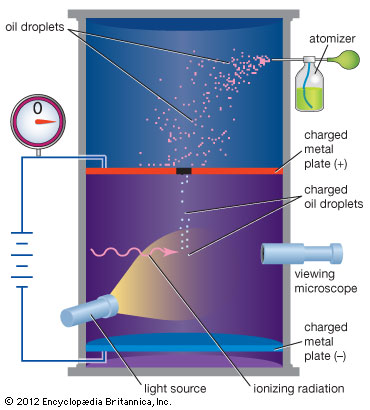
\includegraphics[scale = 0.6]{EM1.jpg}
	\caption{Diagrama de funcionamiento del aparato de Millikan.}
	\label{Fig:a}
\end{figure}
\begin{equation}\label{Ec:1}
	    P_{ap}=P_{gota}-P_{aire}=(p_{agua}-p_{aire})vg
\end{equation}

Finalmente, para el c'alculo de la carga del electr'on ($e$) se toman en consideraci'on la fuerza de gravedad, la intensidad del campo el'ectrico y la ley de Stokes la cual relaciona la velocidad de una esfera en un medio viscoso, teniendo como resultado la siguiente expresión: 
\begin{equation}
   e= \frac{4\pi g\rho d\left(v_{f}+v_{r}\right)\left(\sqrt{\frac{9\eta v_{f}}{2g\rho}+\frac{b^{2}}{4p^{2}}}-\frac{b}{2p}\right)^{3}}{3Vv_{f}}
\end{equation}
en dónde 

\section*{Materiales y equipos}\label{Material}                          	% -------------------- Material
\begin{itemize}
	\item Vernier anal'ogico ($\pm$ 0.025 mm)
	\item Aparato de Millikan ($\pm$ 0.05 mm)
	\item Fuente de alimentaci'on
		\subitem Cable de alimentaci'on 
	\item Mult'imetro ($\pm$ 0.005 Ohms)
	\item 4 Cables banana-banana
\end{itemize}

\section*{Metodolog'ia}\label{Metodologia}				% -------------------- Metodolog'ia

Primeramente, se coloc'o el aparato de Millikan sobre la mesa, situando el alcance de visualizac'on en un lugar permisible sin que se moviera el aparato cuando se observaran las gotas a trav'es de 'el. Con ayuda del nivel de burbuja se nivel'o para que esto no fuera un problema en las mediciones obtenidas.

Despu'es se limpi'o cuidadosamente el aparato, en caso de que hubiera residuos de experimentos anteriores, esto se hizo con ayuda de alcohol isoprop'ilico y toallas de papel Kimtech Science. Posteriormente, con ayuda del vernier, se midi'o el ancho de la placa que separaba las dos placas del capacitor, ya que este representaba la distancia entre ellas. El valor obtenido fue de (0.90 $\pm$ 0.05)cm.

M'as tarde se posicionaron nuevamente las tres placas en su lugar y se conect'o el aparato a una fuente de luz para poder ajustar el enfoque y brillo del alcance de visualizaci'on con ayuda del anillo de enfoque y se apag'o nuevamente el equipo. Inmediatamente despu'es se conect'o a una fuente de alto voltaje DC a los conectores de voltaje. La fuente se ajust'o para que entregaran (500 $\pm$ 5) VDC y tambi'en se conect'o un mult'imetro para corroborar el voltaje suministrado y determinar la resistencia aplicada. La cual fue de (2.1131 $\pm$ 0.0001)\;M$\Omega$. Una vez que se tuvieron todos los elementos en su lugar, se llev'o a cabo el experimento. El arreglo del equipo se muestra en la siguiente figura.

\begin{figure}[H]
	\centering
	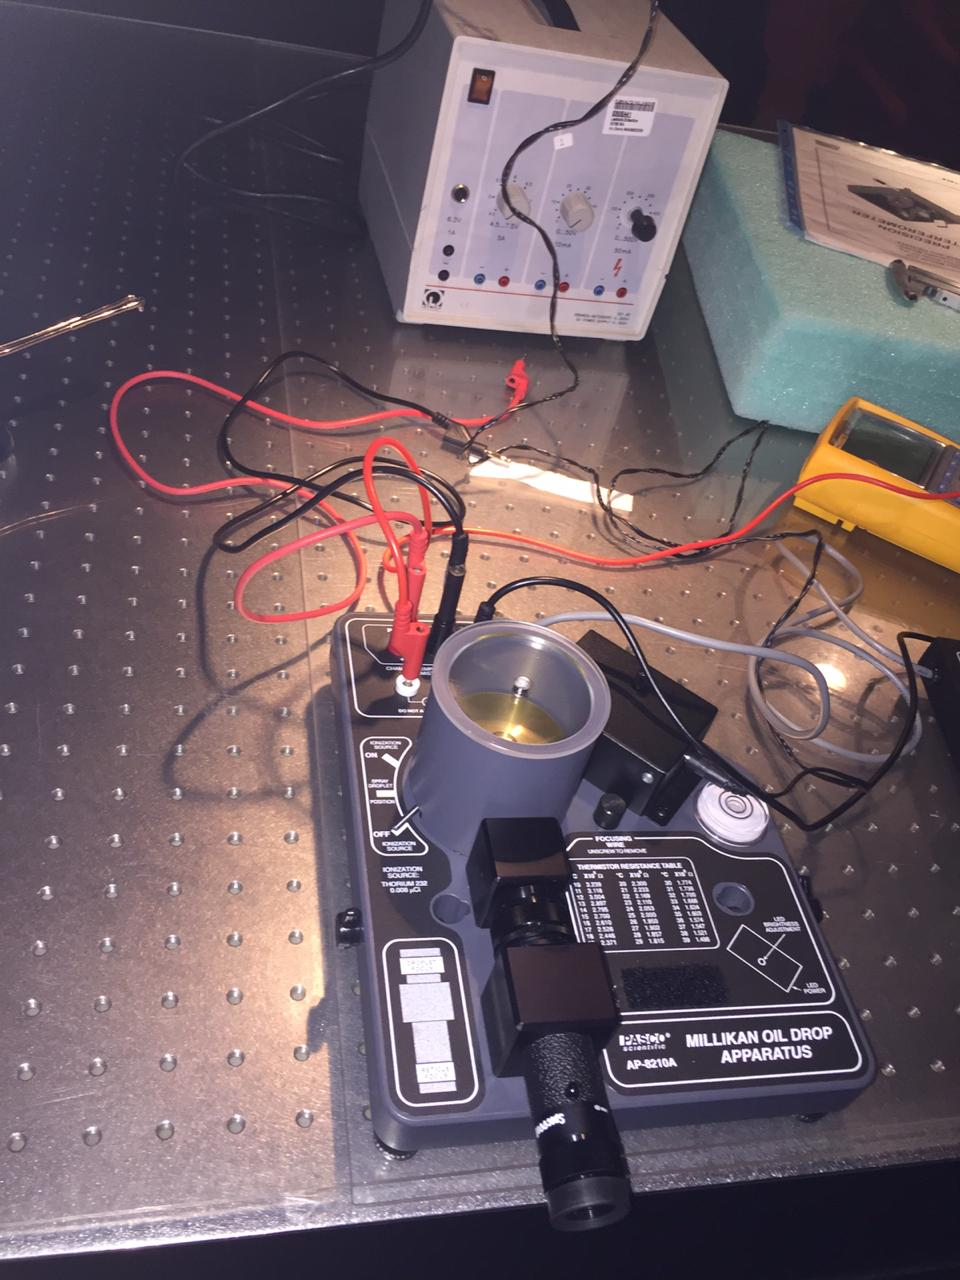
\includegraphics[scale = 0.13]{Milikan-set-up.jpeg}
	\caption{Configuraci'on del equipo del experimento de Milikan.}
	\label{Fig:1}
\end{figure}

Para iniciar con la sección experimental, se asegur'o que la punta del atomizador estuviera apuntando hacia abajo al mismo tiempo que formaba un 'angulo de 90$^{\circ}$ del mango del atomizador. Antes de que se a'nadieran las gotas de aceite al equipo, se preparaba el atomizador apretando r'apidamente la v'alvula del mismo. Una vez que esto ocurr'ia, se pon'ia la palanca de fuente de ionizaci'on en la posic'on "spray droplet position" para que el aire de la c'amara escapara mientras las gotas entraban en ella. Cuando en el lente de visualizaci'on se pod'ia apreciar una lluvia de gotas, se cambiaba la palanca a ON para que fueran ionizadas. Posteriormente se elegi'ia una gota la cual no cayera tan r'apido al mismo tiempo que era brillante y f'acil de identificar, se tomaba el tiempo que tardaba en caer y se registraba una vez que desaparec'ia del campo visual y se producía un campo el'ectrico de modo que las gotas cambiasen su dirección y fueran hacia arriba. Nuevamente se eleg'ia una gota que no pasara r'apidamente frente a la pantalla y fuera brillante, su tiempo contabilizaba y registraba. 'Este proceso se repiti'o al menos 10 veces y los resultados obtenidos son analizados en la siguiente secci'on.

\section*{Resultados y an'alisis}\label{Resultados}
Primeramente, con el valor de la resistencia obtenida se calculó un valor correspondiente de temperatura con ayuda de una tabla que se encontraba incluida. Para un valor $R= (2.1131 \pm 0.0001)M\Omega$ se tiene una temperatura $T=(2.113110 \pm 0.000007)^{\circ}C$, calculada con los valores de la Tabla del apéndice B del manual del aparato. De similar manera, de obtuvo un valor de la viscosidad del aire en función de la temperatura anterior con la gráfica del apéndice A del mismo manual, esta fue
$\eta=(1.83751341\pm0.00000008)\cdot10^{-5}\frac{Ns}{m^2}.$

Para calcular el valor de la velocidad de bajada ($v_f$) y de subida ($v_r$) se midieron los tiempos que les tomaba a tres partículas distintas de aceite recorrer una distancia $d=(1.00\pm0.05)mm$ tanto de subida como de bajada. Los datos obtenidos se muestran en las Tablas 1, 2 y 3 correspondientes a cada gota estudiada.



Con base en cada una de la tablas, se puede calcular una velocidad de bajada y caída promedio, $\overline{v_f}$ y $\overline{v_f}$ respectivamente. Una vez obtenidos estos, podemos calcular el valor de la carga del electrón ($e$) para cada gota.
Estos tres datos se presentan en la Tabla 4.


Este experimento tuv'o, principalmente la aplicaci'on de ayudar a determinar la carga de un electr'on a trav'es de equilibrar la fuerza gravitatoria con la flotabilidad y las fuerzas el'ectricas. Esto a su vez, ayudar'ia a determinar la masa del electr'on con la relación de carga-masa propuesta por Thompson. Asimismo, ayudar'ia a conocer que a nivel de partículas tan pequeñas como las partículas elementales, los efectos gravitatorios son despreciables frente a los electrostáticos. 

Gracias a esto, ha sido posible el poder entender el funcionamiento del mundo at'omico, que a su vez esta abriendo puertas para que se desarrollen materiales qu'imicos, como los nanom'etricos, que pretenden ser ergon'omicos y mejorar la calidad de vida humana. 

\section*{Conclusiones}\label{Conclusiones}			Se considera el experimento no exitoso, pues los resultados obtenidos difieren demasiado con respecto al teórico. Al ser este de $\approx 1.6\cdot10^{-19}C$, y nuestros resultados teniendo un orden de magnitud de diferencia, se obtuvieron errores porcentuales de $761\%,1148\%$ y $1010\%$ para las gotas 1, 2 y 3, respectivamente.

Se considera que esto fue posiblemente causado por diversos factores. Entre ellos, variable que no pudieron ser medidas, como lo fueron la densidad del aceite utilizado y la presión en el ambiente. Este último factor es especialmente apreciable en las mediciones de los tiempos de subida y bajada, porque observamos que ligeras perturbaciones en la presión del aire, tal como las causadas por ruidos, producían cambios de trayectoria notables en las partículas de aceite.
Posiblemente estas afectaciones en las mediciones de los tiempos terminó alterando de gran manera el resultado final.


% ------------------------------------------------------------------------------------------------------------------------------------------------------

\end{multicols}

\end{document}										% -------------------- End Document
